% Template for PLoS
% Version 1.0 January 2009
%
% To compile to pdf, run:
% latex plos.template
% bibtex plos.template
% latex plos.template
% latex plos.template
% dvipdf plos.template

\documentclass[10pt]{article}

% amsmath package, useful for mathematical formulas
\usepackage{amsmath}
% amssymb package, useful for mathematical symbols
\usepackage{amssymb}

% graphicx package, useful for including eps and pdf graphics
% include graphics with the command \includegraphics
\usepackage{graphicx}

% cite package, to clean up citations in the main text. Do not remove.
\usepackage{cite}

\usepackage{color} 

% Use doublespacing - comment out for single spacing
%\usepackage{setspace} 
%\doublespacing


% Text layout
\topmargin 0.0cm
\oddsidemargin 0.5cm
\evensidemargin 0.5cm
\textwidth 16cm 
\textheight 21cm

% Bold the 'Figure #' in the caption and separate it with a period
% Captions will be left justified
\usepackage[labelfont=bf,labelsep=period,justification=raggedright]{caption}

% Use the PLoS provided bibtex style
\bibliographystyle{plos2009}

% Remove brackets from numbering in List of References
\makeatletter
\renewcommand{\@biblabel}[1]{\quad#1.}
\makeatother


% Leave date blank
\date{}

\pagestyle{myheadings}
%% ** EDIT HERE **


%% ** EDIT HERE **
%% PLEASE INCLUDE ALL MACROS BELOW

%% END MACROS SECTION

\begin{document}

% Title must be 150 characters or less
\begin{flushleft}
{\Large
\textbf{ClinicalCodes: An online clinical codes repository to improve validity and reproducability of medical database research}
}
% Insert Author names, affiliations and corresponding author email.
\\
David A Springate$^{1,\ast}$, 
Evan Kontopantelis$^{1}$,
Darren Ashcroft$^{2}$,
Ivan Olier$^{1}$,
Rosa Parisi$^{2}$,
Edmore Chamapiwa$^{1}$,
David Reeves$^{1}$
\\
\bf{1} Centre for Primary Care/Centre for Biostatistics, University of Manchester, Manchester, UK
\\
\bf{2} Manchester Pharmacy School, University of Manchester, Manchester, UK
\\
$\ast$ E-mail: Corresponding david.springate@manchester.ac.uk
\end{flushleft}

% Please keep the abstract between 250 and 300 words
\section*{Abstract}

Lists of clinical codes are the foundation for electronic medical record studies and without access to them, reviewers are unable to determine the validity of research, true replication is impossible and researchers are unable to make effective comparisons between studies and are subject to much duplication of effort in building new code lists.  Despite this, publication of clinical codes are not a requirement for obtaining grants, validating protocols or publishing research.  We have built a centralised online repository where electronic medical records researchers can upload and download clinical codes to help address these problems.  The repository will enable clinical researchers to better validate electronic medical records studies, build on previous code lists and compare disease definitions across studies.  It will also assist health informaticians in replicating database studies, tracking changes in disease definitions or GP coding practice through time and sharing clinical code information across platforms and data sources as research objects. 

\section*{Introduction}

Over the last 20 years, increasing numbers of general practicioners have used computers to store patients medical records for various administrative functions \cite{Purves1996}. Hospitals are also beginning to store their records electronically, though electonic hospital records are far less prevelant than in primary care \cite{Ashish2009}. These electronic medical records (EMRs) offer great potential for research, enabling the rapid identification of patients for inclusion in intervention and observational studies. As their use becomes more widespread, it is becoming more important to understand the threats to the validity of research using EMR data. EMRs are being used by researchers to address important questions in healthcare that would be difficult or impossible to address using randomised controlled trials, beacuse of the costs involved, the low prevelance of conditions or beacuse a condition may occur in a subgroup such as children or pregnant women. In UK primary care in particular, the annual number of research outputs based on the three main UK primary care databases (The Clinical Practice Research Datalink (CPRD, formerly the General Practice Research Database, GPRD), The Health Improvement Network (THIN) and QResearch) appears to be increasing at an exponential rate (figure \ref{figure1_articles_per_year}). 


Much research has been done into establishing the internal and external validity of EMR studies \cite{Herrett2010}, particulary from the point of view of data quality, data completeness and confounding.  There has also been work replicating studies from one PCD in another to test if the ...

However, even if all of these issues are adequately addressed, most studies still assume that the underlying definitions of clinical entities (such and conditions, treatments and comorbidities) are valid.  In most cases it is impossible to determine wheter this is in fact the case. 

Clinical entities in PCDs are entered by general practicioners as clinical codes.  In UK primary care, Read codes are the most commonly used clinical code, but others include SNOMED and ICD-9/10.  These codes form a hierarchical classification system which can be used to define symtoms, signs and diagnoses, referrals to hospitals and clinics, immunisation records, prescription information and diagnostic test results.


But the process of preparing such code-lists is far from straightforward, and lacks rigour. The same clinical condition can be described using many different codes. A patient with a given clinical condition might receive one of several possible diagnostic codes as well as, or instead of, one or more codes describing symptoms or investigations. This flexibility in the coding structure facilitates the clinical use of these codes, minimising the time spent searching for codes by practitioners. However, this multitude of codes for a given condition presents a challenge when data need to be aggregated.

The process of drawing up code-lists to identify all patients with a given clinical condition is a critical step in EMR studies and multiple code-lists may be required within one study for many different conditions such as co-variates and confounders as well as disease outcomes.  However, this is often a complicated and time-consuming process involving defining the clinical entity of interest and iteratively searching for codes in lookup tables, running searches for codes in different sections of the database, collating the results and classifying them (generally by clinically trained investigators) \cite{Nicholson2013}.  The built in flexibility and redundancy of clinical coding systems allows practicioners to use a variety of codes to describe a given condition and minimises their time spent searching for codes, but it presents a challenge to researchers using these codes to effectively define a condition.  Also, there could be a combination of diagnostic codes, symtoms, drugs and tests which in combination give a description of the nature of a conditon in a patient. 


The selection of codes used to identify condition and comorbidities will vary according to the particular research question being asked, partly reflecting the degree of certainty of diagnosis required. Sometimes it may be important to identify all possible cases but at other times the study population may need to be restricted to cases where diagnosis is more certain. This variability in code-lists may have major implications for results of all studies using EMRs \cite{Nicholson2011}. For example, a sevenfold variation in estimates of incidence of rheumatoid arthritis can be largely explained by differences in code-lists \cite{Garcia2009, Watson2003}.  Other studies have used different subsets of code-lists in sensitivity analyses \cite{Doran2011, Herrett2010}.  Futhermore and in particular for uncommon diseases, small errors code selection can result in large numbers of misclassified patients, leading to biased results and classification errors affecting conclusions in unpredictable ways \cite{Manuel2010}. The use of different clinical codes may also change over time (for example to keep up with changing guidelines such as the UK Quality and Outcomes Framework) \cite{Gulliford2009}.  Finally, Different researchers may have different intepretations of the relevance of particular codes.

Despite the importance of code-list validity, and calls for sharing of code-lists and greater transparency in the selection of code lists and reporting of sensitivity analyses using different sets of codes\cite{Gulliford2009, Bhattarai2012}, code-lists are still seldom reported in papers \cite{Herrett2010}.  There is also currently no obligation on researchers to publish their code lists by funding bodies, journals or regulators.  Furthermore, there is no centralised repository to hold lists of clinical codes.

We identify four main consequences of lack of transparency of clinical code lists.  First, if code lists are not available and not expected to be published alongside the primary research using them, they represent an important part of a study methodology that is not subject to scrutiny or peer review. In the extreme case, there is no way to determine if a condition diagnosis in a study is valid and clinical decisions could be based on the invalid assumptions drawn from an invalid diagnosis.  This could happen despite rigourous downstram statistical analysis.  Second, the effective replication of EMR studies is dependent on the availability of the clinical codes in the original study.  If all of the codes are not available, it is impossible to tell if differences found in study replications are due to artifactual differences in code lists or if they are genuine.  Third, if code-lists are unknown, comparisons between studies on the same condition are potentially invalidated.  Condition definitions change over time and GP coding practice may also change with respect to regulations and incentives [REF?]. Also, different studies may use different indicator markers for a condition (test scores, drugs, symptoms etc).  Not having access to code-lists means that it is difficult to know whether fair comparisons are being made between paper. Fourth, building code lists for known conditions from scratch is a time consuming process. Having access to historical code-lists  for a condition would mean that new lists could be built incrementally and iteratively, saving much 'reinvention of the wheel'.

To highlight the problem of lack of transparency in clinical code-lists, we look at a representative random sample of UK primary care database studies and identify which studies provide any or adequate detail on clinical coding strategy and access.

To address the issue outlined above and to facilitate transparancy, sharing and retrival of code-lists, we developed ClinicalCodes, a web repository for EMR researchers to freely upload and download clinical code-lists. The collection  of information in a single centralised repository will aid the accessibility of the resource for the benefit of all EMR researchers.

% Results and Discussion can be combined.
\section*{Results and Discussion}

\subsection*{Exploration of the current literature}

Primary care database studies form a large component of total EMR research, and UK PCDs are among the most researched in the world.  Figure \ref{figure1_articles_per_year} shows that research interest in UK PCDs is increasing at an exponential rate, while figure \ref{figure2_PCD_map} shows that research into UK PCDs is being conducted in universities and research hospitals around the world, rather than being limited to the UK.  Because UK PCDs are such a common subject and also the cutting edge  of EMR research, it seems reasonable to expect the levels of transparency of code-lists in UK PCD studies to be no lower than in other EMR studies.  We took a sample of 450 papers from the original 1359 output from the PubMed search.  Of these, 392 (87\%) had both  the full text accessible to the Manchester University library and were examples of primary PCD research.  Of these 392, less than 9% published the entire set of clinical codes needed to reproduce the study in an online appendix and only 12% stated that the clinical codes are available upon request \ref{tab:table1_percentages}.


\subsection*{Database Content}

The main ClinicalCodes database consists of Articles containing metadata such as citation details and abstracts.  Code-lists are associated with these and individual clinical codes with the code-lists. All clinical codes are given a code name, coding system (e.g. Read, SNOMED), description and entity type (e.g. diagnostic, drug code).  Users are able to upload additional data for codes as either supplementary fields for individual codes or as comments at the code-list or article level.  Code lists can be downloaded by any users but an account must be created to upload article metadata or codelists or to leave comments. Code lists can be downloaded in aggregate as a zip file or individually as csv files.  Code lists can be recycled from previous studies by linking to the previous code list.  This reduces workload in uploading lists that are unchanged from previous studies while retaining information on the origin of code lists.  At the time of publication, we have uploaded the complete code lists used for two papers from our group \cite{Doran2011, Kontopantelis2014} as well as codes from the UK Quality and Outcomes Framework Business rules versions 5 and 24 - a total of 13191 clinical codes across 97 code lists.

%%%  RECYCLING CODELISTS FEATURE IS STILL TO BE IMPLEMENTED!   %%%    


\subsection*{Clinical Codes as research objects}

%%%% ro stuff not yet implemented in ClinicalCodes.. %%%%

Research objects are annotated aggregations of data often associated with a scientific publication that facilitate reuse and reproducibility of scientific research \cite{Bechhofer2010}. Following this model, codelists for a specific article are available as research objects that can be shared across platforms in machine readable form.  In practice, this means that a JSON manifest file is available for each article containing: Article metadata (title, author, abstract, reference, link, doi), article level comments, codelist level comments, individual codes with metadata and additional note columns. These files are either stored in a hidden .ro file within the downloaded zip file or are available directly by adding a manifest.json to the URI for an article (e.g. www.clinicalcodes.org/medcodes/article/5/manifest.json).  The research object format is designed to be available without getting in the way of the main method of download that will be required by most users.

\subsection*{Conclusions}

% Biosharing.org
% re3data.org
% force11.org

Large medical datasets, including medical records datasets are already playing an important role in clinical research and this role is set to grow in the era of big data in healthcare \cite{Wang2013}. The continuing success of big data in healthcare will depend on the ability of researchers to leverage, and validate that data and then combine it with other sources \cite{Murdoch2013}.  We have developed a repository for clinical codes that will be of great use to two groups of researchers.  First, clinical researchers using primary care and other medical databases will be able to more effectively validate their research, build upon previous code lists and match appropriate disease definitions through time. Second, health informaticians and meta analysts will more easily be able to produce study replications (e.g. replications across databases such as \cite{Reeves2014}), share clinical code data as research objects across platforms and data sources and use the ClinicalCodes database as an object of research in its own right (e.g. to track changes in disease definitions and doctors' coding practice through time).

There are several motivations for researchers to deposit their codes in the ClinicalCodes repository.  Most importantly, we have endeavoured to make the upload and download processes as painless as possible.  In particular, download of individual codelists is a one-click operation requiring no log in or provision of user information.  Other important incentives include the promise of faster and more consistent development of new code lists, improvements in research quality associated with better scrutiny of lists of clinical codes, greater exposure and potential for studies with uploaded codes to be more highly cited and also providing a way to discover other researchers working in the same area.

Despite these motivations, the success of this project will depend on its adoption by the electronic medical records research community. Although ClinicalCodes solves the problem of having a centralised repository for holding codes, the problem remains that funding bodies, database regulators and journals do not require making clinical code lists accessible. There is a gradual movement towards more transparency and openness in academic research (particularly in disciplines where there is high computational load) at the levels of academic research \cite{Bechhofer2013, Stodden2013, Pampel2013}, learned societies \cite{RoyalSoc2012} and government \cite{EuropeanCommission2012, OfficeSciTech2013}. We believe that adoption and support of a centralised clinical codes repository by the bodies with a vested interest in electronic medical records research will be of great benefit to electronic medical records research.


\subsection*{Availability and Requirements}

%%% Not yet indexed....  %%%%

ClinicalCodes is freely accessable at http://www.clinicalcodes.org and is indexed at www.re3data.org \cite{Pampel2013}.

% You may title this section "Methods" or "Models". 
% "Models" is not a valid title for PLoS ONE authors. However, PLoS ONE
% authors may use "Analysis" 
\section*{Materials and Methods}

\subsection*{Article Classification}

To get an estimate of the extent of the problem of lack of transparency in clinical code-lists in EMR studies, we collected articles conducting primary research using the three major UK-wide Primary care databases (PCDs) (The Clinical Practice Research Datalink, formerly the General Practice Research Database; The Health Improvement Network; QResearch).  The UK has one of the most extensive and longest running systems of collection of EMRs and The main UK PCDs are the subject of considerable research interest.  A Search was made on Pubmed for articles with the following terms: ``CPRD'', ``Clinical Practice Research Datalink'', ``GPRD'', ``General Practice Research Database'', ``The Health improvement Network'', ``QResearch''.  A random sample of $1/3$ of the Pubmed search was taken for further analysis.  From this sample, all articles were identified that were both primary EMR research and had their fulltext accessable via the University of Manchester library. We then scored each paper as belonging or not to the following categories:

\begin{enumerate}
    \item Are any clinical codes listed in the methods section?
    \item Is at least one full code list provided in the paper or in an appendix?
    \item Are all code lists provided to enable replication of the study?
    \item Is it stated that ``Code lists are available on request''? 
\end{enumerate}

All analyses were performed using R v2.15.2 \cite{R2012}. Article counts over time and geocoded article affiliations (Via the Google Geocoder API) were aggregated using the R package rpubmed (https://github.com\slash ropensci/rpubmed).

\subsection*{Database Architecture and Web Interface}

The back end data is stored in a relational database called PostgreSQL (http://www.postgresql.org). Server-side web programming was done in Python v2.7.5 (http://www.python.org) using the Django v1.5 web framework (https://www.djangoproject.com). The client side scripting was done in JavaScript and HTML5 and used Twitter Bootstrap v3 (http://getbootstrap.com) as a front-end framework.  The dynamic parts of the site were served using Gunicorn v18.0 (http://gunicorn.org) and static parts with Nginx v1.0.15 (http://nginx.org). Cacheing and sessions are handled by a Redis v2.4.10 NoSQL database (http://redis.io). The repository is hosted on a 64 bit Red Hat Enterprise Linux server release 6.4 virtual machine  at the University of Manchester. 


% Do NOT remove this, even if you are not including acknowledgments
\section*{Acknowledgments}
We are thankful to Matt Ford for extensive technical support. Thanks to the Research team at CPRD for fruitful discussions in the development stage.  This work was supported by...

\section*{Author Contributions}

Conceived, designed and built the repository: DAS. Data collection DAS, DR, EK, IO, RP, DA, EC.  Data Analysis DAS. Wrote the paper DAS ...

%\section*{References}
% The bibtex filename
\bibliography{clinicalcodes}

\section*{Tables}

\begin{table}[!ht]
  \caption{
    \bf{Percentages of a random sample of UK primary care database studies with details of code lists}}
  \begin{tabular}{|c|c|c|}
    \hline
                 & Number of articles & Percentage \\
    \hline
    All UK PCD articles        & 1359 & ---  \\
    In random sample           & 450  & ---  \\
    Full-text available        & 417  & ---  \\
    Primary PCD research       & 392  & 100  \\
    Any code in methods        & 104  & 26.5 \\
    Any code list in study     & 74   & 18.9 \\
    All relevant code-lists    & 34   & 8.7  \\
    Any codes in paper         & 117  & 29.8 \\
    Codes available on request & 48   & 12.2 \\
    Any codes or available     & 138  & 35.2 \\
    \hline
  \end{tabular}
  \begin{flushleft}Percentages are relative to the number of primary PCD research studies 
  \end{flushleft}
  \label{tab:table1_percentages}
\end{table}


\section*{Figure Legends}

\begin{figure}[!ht]
\begin{center}
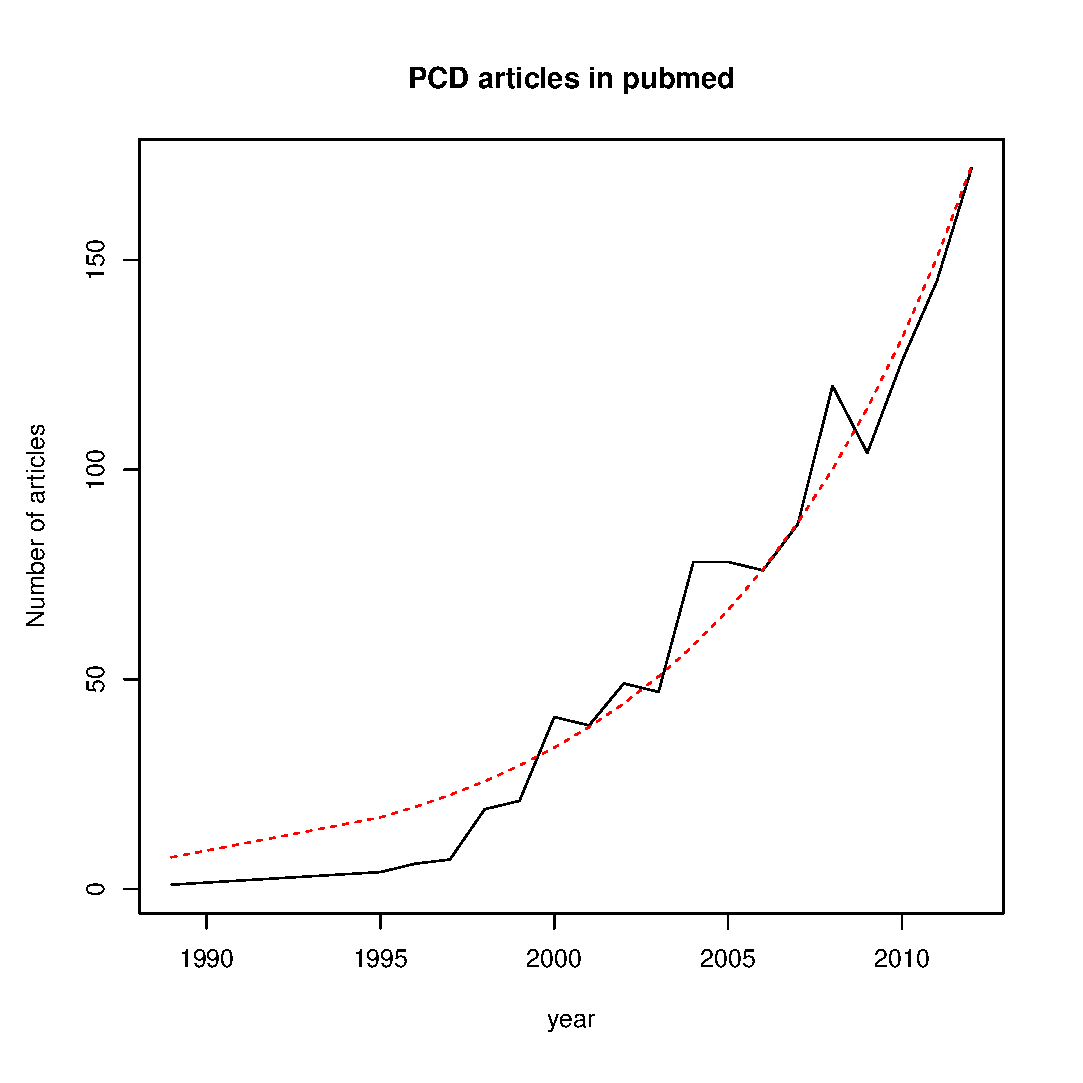
\includegraphics[width=4in]{figure/articles_per_year.eps}
\end{center}
\caption{
    {\bf Number of UK Primary Care Database publications.}
}
\label{figure1_articles_per_year}
\end{figure}

\begin{figure}[!ht]
\begin{center}
  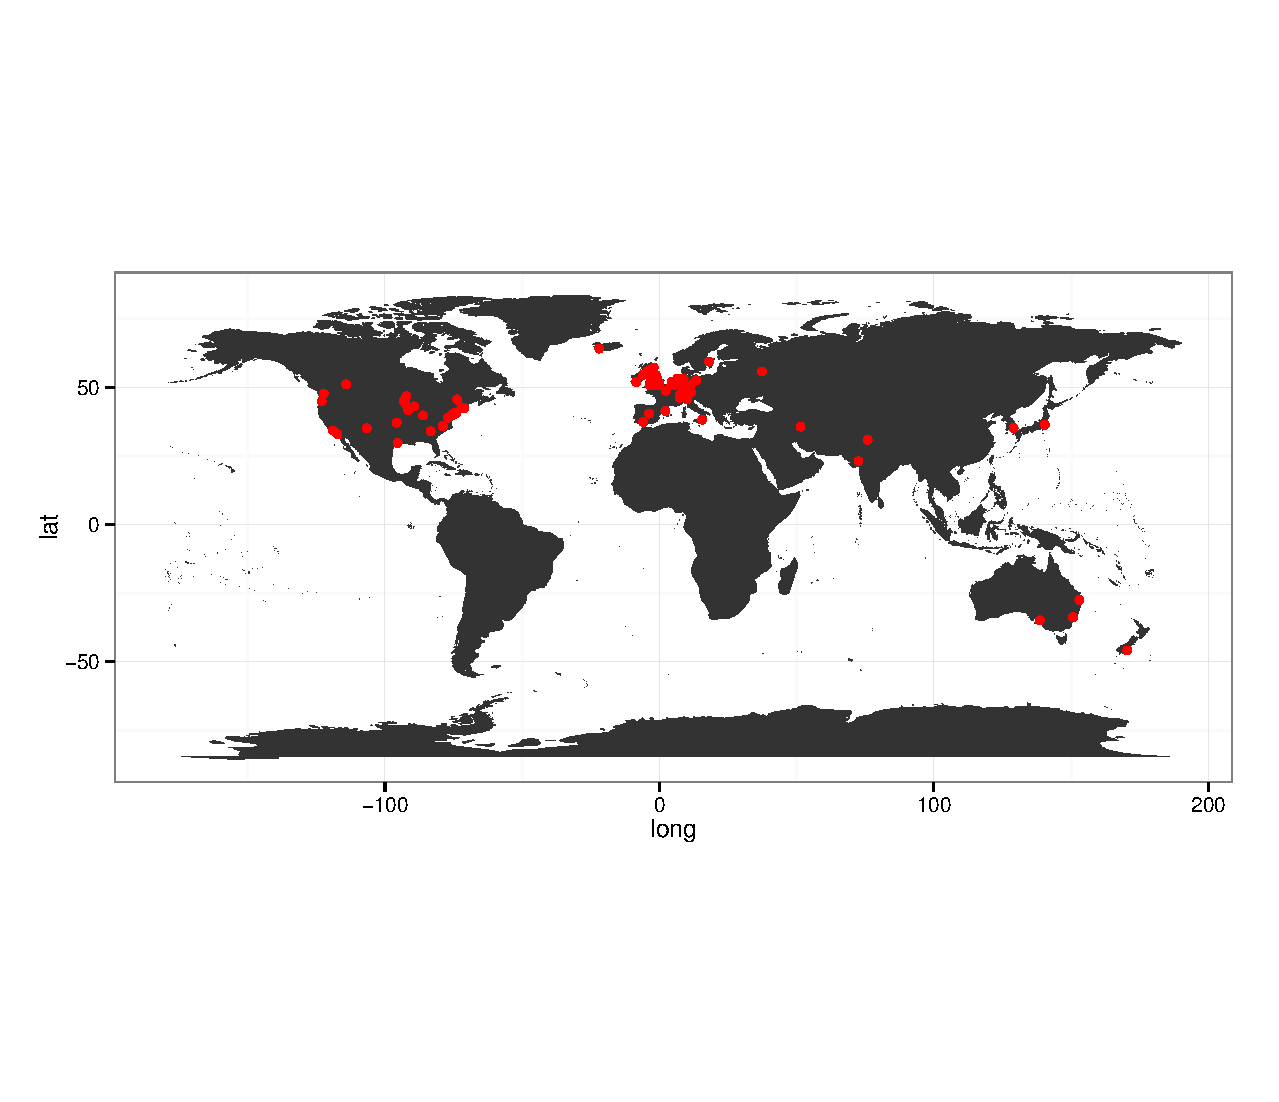
\includegraphics[width=4in]{figure/PCD_world.eps}
\end{center}
\caption{
    {\bf Locations of primary affiliated departments.}
}
\label{figure2_PCD_map}
\end{figure}

\end{document}

